\documentclass[conference]{IEEEtran}

\usepackage{amsmath,amssymb,amsfonts}
\usepackage{graphicx}
\usepackage{booktabs}
\usepackage{multirow}
\usepackage{cite}
\usepackage{url}
\usepackage{xcolor}
\usepackage{bm}
\usepackage{siunitx}
\usepackage{tikz}
\usepackage{amsthm}
\usepackage{algorithm}
\usepackage{algorithmic}
\usetikzlibrary{arrows.meta,positioning,fit,backgrounds,calc,decorations.markings}

\newcommand{\SO}{\mathrm{SO}(3)}
\newcommand{\se}{\mathfrak{se}(3)}
\newcommand{\R}{\mathbb{R}}
\newcommand{\xhat}{\hat{\mathbf{x}}}
\newcommand{\bvec}[1]{\mathbf{#1}}
\newtheorem{proposition}{Proposition}
\newtheorem{lemma}{Lemma}
\newtheorem{theorem}{Theorem}

% Compact float and equation spacing for RA-L 8-page format
\setlength{\textfloatsep}{4pt plus 1pt minus 1pt}
\setlength{\floatsep}{4pt plus 1pt minus 1pt}
\setlength{\intextsep}{4pt plus 1pt minus 1pt}
\setlength{\abovedisplayskip}{3pt plus 1pt minus 1pt}
\setlength{\belowdisplayskip}{3pt plus 1pt minus 1pt}
\setlength{\abovedisplayshortskip}{1pt plus 1pt minus 1pt}
\setlength{\belowdisplayshortskip}{1pt plus 1pt minus 1pt}

\begin{document}

\title{HD-LIO: Three-Level Hierarchical Surfel Map\\with Degeneracy Feedback for Drift-Resilient\\LiDAR-Inertial Odometry}

\author{[Author names withheld for review]%
\thanks{Manuscript received [date]; revised [date].}%
\thanks{[Affiliation and address]}%
\thanks{Corresponding author: [email]}%
}

% \markboth removed for conference format

\maketitle

\begin{abstract}
Tightly coupled LiDAR-inertial odometry (LIO) is widely adopted for
autonomous navigation, yet its performance remains sensitive to
geometric degeneracy that arises in confined corridors, planar regions,
and narrow field-of-view (FOV) sensors. While prior degeneracy-aware
methods detect rank deficiency in the estimator, the underlying map
representation continues to absorb drifted points one-way, allowing a
\emph{drift-map positive feedback loop} that, to our knowledge, has not
been explicitly modeled in tightly coupled LIO. To address this issue,
we propose HD-LIO, a tightly coupled LIO framework designed around
\emph{bidirectional estimator--map feedback} along rank-deficient
directions. HD-LIO comprises three key components.
First, we formalize the drift-map positive feedback as a per-direction
linearized recursion $\epsilon_{k+1} = [1 + \alpha(\bvec{n}\!\cdot\!\bvec{d})^2]\epsilon_k + O(\alpha^2)$,
exposing the map's learning rate $\alpha$ as the controllable amplification
gain, and derive sufficient conditions under which map-side feedback
yields ultimate-bounded drift on the subset of frames satisfying these
conditions ($\ge\!96.8\%$ on indoor Avia).
Second, inspired by this analysis, we propose a three-mechanism
degeneracy response—learning-rate modulation, source switching, and
write gating—operating at distinct points of the loop on a hierarchical
surfel map that provides persistent surface statistics for temporal
smoothing and information-matrix stabilization.
Third, to inject map-aware reliability into the iterated Kalman update,
we derive a closed-form per-correspondence weight $\sigma^2_n =
\lambda_0/(N_c\lambda_2)$ from eigenvalue perturbation theory under
explicit assumptions, and incorporate it into the IEKF residual
covariance.
HD-LIO is evaluated across three LiDAR types (NTU OS1-16, Avia,
Mid-360) over 35 unique trajectories, recorded as 43 sensor-bag pairs
(8 indoor trajectories carry both Avia and Mid-360 recordings). On the
35 baseline-comparable bags, HD-LIO achieves \SI{0.203}{\meter} uniform
per-bag mean ATE---the lowest mean on each of the four dataset
groups---and, on the additional 8~indoor Avia bags (70\textdegree{} FOV)
where all six evaluated baselines diverge ($\mathrm{ATE}{>}\SI{10}{\meter}$),
HD-LIO is the only method among the evaluated baselines to maintain
bounded error. Ablation reveals
FOV-dependent activity: degeneracy feedback dominates under narrow
FOV ($+$53\% with removal), is largely dormant under 360\textdegree{}
($\le 1$\% impact), and the surfel map prevents divergence under
severe occlusion ($+$185\% mean ablation, driven by a single
Mid-360 outlier); the proposed FOV-adaptive framework
handles this regime separation without per-scene reconfiguration.
\end{abstract}

\begin{IEEEkeywords}
LiDAR-inertial odometry, hierarchical surfel map, degeneracy detection,
iterated Kalman filter, normal uncertainty
\end{IEEEkeywords}

%----------------------------------------------------------------------
\section{Introduction}\label{sec:intro}
%----------------------------------------------------------------------

LiDAR-Inertial Odometry (LIO) has been actively developed over the past
decade for autonomous navigation across diverse
environments~\cite{xu2021fastlio,xu2022fastlio2,bai2022fasterlio,
chen2024iglio,he2023pointlio,shan2020liosam,chen2023dlio}. Despite
this progress, LIO performance has been observed to degrade in response
to two key geometric characteristics of the surrounding environment:
(i) the \emph{rank deficiency} of the local information matrix in
confined corridors, planar regions, and feature-sparse open spaces; and
(ii) the \emph{LiDAR field-of-view (FOV) regime}, which determines how
much the rank deficiency in (i) propagates into the estimator. For
narrow-FOV solid-state LiDARs such as the Livox Avia ($70^\circ$),
even outdoor scenes routinely exhibit at least one degenerate direction
in 58\% of frames in our dataset, indicating that geometric degeneracy
is a regime to be designed for, not a corner case.

Existing tightly coupled LIO systems—FAST-LIO2~\cite{xu2022fastlio2}
(ikd-tree~\cite{cai2022ikdtree}), Faster-LIO~\cite{bai2022fasterlio}
(flat voxel hash), iG-LIO~\cite{chen2024iglio} (GICP-cost covariance),
and VoxelMap~\cite{yuan2022voxelmap} (adaptive plane parameters)—evolve
their map content based on incoming points, but the map's update rule
itself is not modulated by the estimator's per-direction confidence. Estimator-side
degeneracy methods such as Zhang and Singh's
factor~\cite{zhang2016degeneracy} and X-ICP/Lodestar~\cite{li2025lodestar}
gate or project the state update along rank-deficient directions but
leave the map's learning rate $\alpha$ unchanged, so drifted points
are still absorbed at full rate and contaminate subsequent
correspondences. This estimator-only intervention point allows a
\emph{drift-map positive feedback loop} which, to our knowledge, has
not been explicitly formalized as a per-direction recursion or
addressed via direction-selective map-side feedback in prior tightly
coupled LIO work (Sec.~\ref{sec:degen}).

For these reasons, we seek a tightly coupled LIO framework that
operates robustly not only in narrow- and full-FOV outdoor scenes but
also under indoor degeneracy where rank deficiency is sustained.
To this end, we propose a generalizable framework, called HD-LIO,
designed around two guiding principles:
(i)~\emph{bidirectional estimator--map feedback} along rank-deficient
directions, and
(ii)~\emph{per-correspondence reliability} informed by local
measurement uncertainty.

Building on prior surfel-based map representations~\cite{behley2018suma,
yuan2022voxelmap} and eigenvalue perturbation theory~\cite{stewart1990matrix},
HD-LIO contributes an FOV-adaptive intervention that breaks the loop at
three distinct points, rather than introducing a new map data
structure or noise model in isolation. To realize the first principle, the three mechanisms operate
at distinct points of the recursion: the map's learning rate $\alpha$
is modulated along degenerate directions, the correspondence source is
switched between surfel-cached planes and a Per-query Voxel Map (PVMap)
when the surfel pathway becomes unreliable, and write operations into
the PVMap ring buffer are gated by the same alignment criterion. To
realize the second principle, HD-LIO derives a closed-form
per-correspondence weight $\sigma^2_n$ under explicit assumptions and
injects it into the IEKF as residual covariance, making the update
aware of local surface quality.

We make four claims, backed by the subsequent sections and our
experimental evaluation: (i)~we formally model the drift-map positive
feedback loop in tightly coupled LIO and derive sufficient conditions
for ultimate-bounded drift under map-side feedback; (ii)~we propose a
three-mechanism degeneracy response operating at distinct points of
the loop, integrated with a hierarchical surfel map; (iii)~we derive
an approximate closed-form per-correspondence weight under explicit
assumptions; (iv)~we evaluate across 35 unique trajectories (43 sensor-bag pairs)
on three LiDAR types, achieving the lowest mean ATE in each evaluated
regime relative to the six compared baselines, with the strongest
margin on NTU~VIRAL (9/9 best, 22\% below LIO-SAM).

%----------------------------------------------------------------------
\section{Related Work}\label{sec:related}
%----------------------------------------------------------------------

We review three pillars relevant to the present work: tightly-coupled
LIO systems, map-derived measurement uncertainty, and degeneracy
handling.

\textbf{LIO systems and map representations.}
Building on LOAM~\cite{zhang2014loam}, FAST-LIO/FAST-LIO2~\cite{xu2021fastlio,
xu2022fastlio2} replaced feature extraction with direct point-to-plane
registration against an ikd-tree~\cite{cai2022ikdtree} via a
tightly-coupled IEKF on manifold IMU
preintegration~\cite{forster2017manifold}. Point-LIO~\cite{he2023pointlio}
processes individual points for per-point updates; Faster-LIO~\cite{bai2022fasterlio}
replaces the ikd-tree with incremental voxels; LIO-SAM~\cite{shan2020liosam}
integrates LIO within a factor graph~\cite{dellaert2017factor};
DLIO~\cite{chen2023dlio} adds continuous-time motion
correction~\cite{dellenbach2022cticp}. A common characteristic across
these systems is that the map functions as a passive data store that
does not adapt its behavior to the estimator's confidence.
We note that LiDAR-only ICP-class methods such as
KISS-ICP~\cite{vizzo2023kissicp}, CT-ICP~\cite{dellenbach2022cticp},
and MAD-ICP~\cite{ferrari2024madicp} fall outside the tightly-coupled
LIO scope of this paper, as they do not perform IMU--LiDAR fusion
within a single Bayesian filter and therefore cannot exploit the
high-rate IMU prior that anchors the per-direction noise weighting in
Sec.~\ref{sec:framework}.

\textbf{Map-derived measurement uncertainty.}
Censi~\cite{censi2007accurate} derived closed-form covariance for ICP;
Segal et~al.~\cite{segal2009gicp} formulated GICP with local Gaussian
distributions, extended to voxelized representations by
Koide et~al.~\cite{koide2021vgicp} (see~\cite{pomerleau2015review} for
a survey). VoxelMap~\cite{yuan2022voxelmap} maintains adaptive
probabilistic plane models within a voxel hierarchy, and
iG-LIO~\cite{chen2024iglio} integrates incremental GICP into a
tightly-coupled IEKF; both, however, embed covariance in the GICP
\emph{cost function} rather than as the IEKF measurement noise
$R_\mathrm{m}$ that modulates the Kalman gain.
Surfel-LIO~\cite{lv2025surfellio}, extending the surfel-based mapping
paradigm~\cite{behley2018suma} to LIO, caches surfel descriptors for
fast queries with planarity-based gating but does not propagate the
surfel eigenspectrum into the per-correspondence noise model used by
the filter. While prior LIO/ICP variants employ range-dependent or
GICP-cost covariances, to our knowledge no surveyed system derives a
\emph{closed-form surfel-eigenspectrum-based} angular uncertainty
$\sigma^2_n{=}\lambda_0/(N_c\lambda_2)$ and injects it as an explicit
per-correspondence IEKF residual covariance weight.

\textbf{Degeneracy detection and handling.}
Zhang et~al.~\cite{zhang2016degeneracy} provided the foundational
analysis, projecting the solution away from under-constrained
directions identified through eigenvalue decomposition of the Hessian.
LODESTAR~\cite{li2025lodestar} freezes degenerate state components via
a Schmidt-EKF, while X-ICP~\cite{tuna2024xicp} introduces per-direction
localizability analysis and DARE-SLAM~\cite{ebadi2021dareslam} applies
eigenvalue-based mitigation in multi-robot settings.
All of these methods confine degeneracy handling to the estimator: the
state update is modified, but the map continues to absorb potentially
drifted points, creating the positive feedback loop that
Sec.~\ref{sec:degen} formalizes.

%----------------------------------------------------------------------
\section{System Overview}\label{sec:overview}
%----------------------------------------------------------------------

\noindent
HD-LIO follows the dual-source IEKF paradigm of FAST-LIO2-class
systems but augments the map with bidirectional feedback to break the
drift-map positive feedback loop introduced under geometric
degeneracy (formalized in Sec.~\ref{sec:degen} as
Eq.~\eqref{eq:drift_feedback}). The system breaks this loop at three
distinct points—the map's learning rate, the correspondence source,
and the write policy—each operating on a hierarchical surfel
representation that decouples per-scan amplification from across-scan
accumulation; Sec.~\ref{sec:stability} proves the resulting drift is
ultimately bounded under explicit conditions on geometric diversity
and prior-uncertainty matching.

\begin{figure*}[t]
  \centering
  \resizebox{\textwidth}{!}{%
  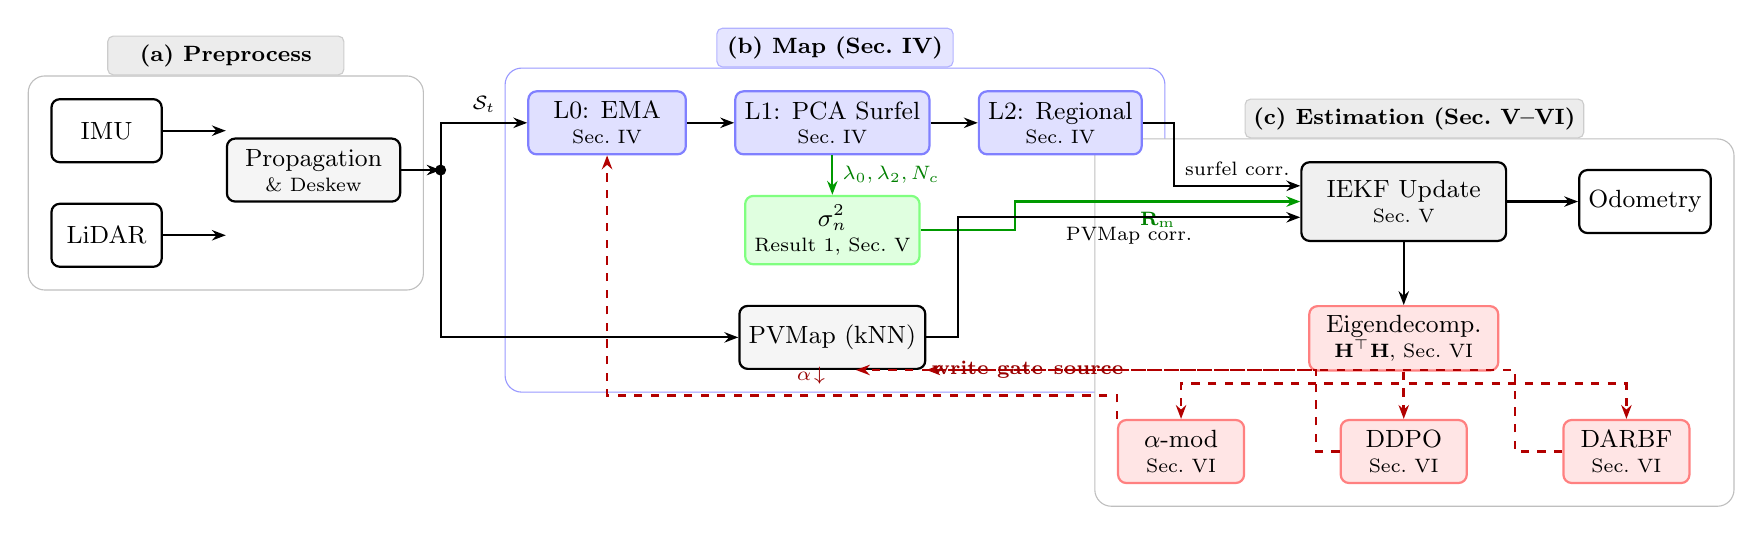
\begin{tikzpicture}[
    node distance=0.55cm and 0.7cm,
    baseblock/.style={draw, rounded corners=3pt, minimum height=0.8cm,
                      font=\small, align=center, thick},
    stdblock/.style={baseblock, fill=gray!8, minimum width=1.6cm},
    mapblock/.style={baseblock, fill=blue!12, draw=blue!50, minimum width=2.0cm},
    uncblock/.style={baseblock, fill=green!12, draw=green!50, minimum width=1.8cm},
    fbblock/.style={baseblock, fill=red!10, draw=red!50, minimum width=1.6cm},
    ioblock/.style={baseblock, fill=white, minimum width=1.4cm},
    arrow/.style={-{Stealth[length=5pt]}, thick},
    dataarrow/.style={arrow, black},
    uncarrow/.style={arrow, green!60!black, thick},
    fbarrow/.style={-{Stealth[length=5pt]}, thick, dashed, red!70!black,
                    line width=1.0pt},
    lbl/.style={font=\scriptsize},
    lblgreen/.style={font=\scriptsize\bfseries, green!50!black},
    lblred/.style={font=\scriptsize\bfseries, red!60!black},
    secheader/.style={font=\footnotesize\bfseries, rounded corners=2pt,
                      inner sep=3pt, minimum width=3.0cm, anchor=south},
  ]
    % (a) Preprocess
    \node[ioblock] (imu) {IMU};
    \node[ioblock, below=0.5cm of imu] (lidar) {LiDAR};
    \node[stdblock, right=0.8cm of imu, yshift=-0.5cm, minimum width=2.2cm]
          (prop) {Propagation\\[-2pt]{\scriptsize\& Deskew}};
    \draw[dataarrow] (imu.east) -- (prop.west|-imu.east);
    \draw[dataarrow] (lidar.east) -- (prop.west|-lidar.east);

    % (b) Hierarchical Surfel Map
    \node[mapblock, right=1.6cm of prop, yshift=0.6cm] (l0)
          {L0: EMA\\[-2pt]{\scriptsize Sec.~IV}};
    \node[mapblock, right=0.6cm of l0] (l1)
          {L1: PCA Surfel\\[-2pt]{\scriptsize Sec.~IV}};
    \node[mapblock, right=0.6cm of l1] (l2)
          {L2: Regional\\[-2pt]{\scriptsize Sec.~IV}};
    \node[uncblock, below=0.5cm of l1] (sigman)
          {$\sigma^2_n$\\[-2pt]{\scriptsize Result~1, Sec.~V}};
    \node[stdblock, below=0.5cm of sigman, minimum width=2.0cm] (pvmap)
          {PVMap (kNN)};

    % Fork point from Propagation
    \coordinate (fork) at ([xshift=0.5cm]prop.east);
    \draw[dataarrow] (prop.east) -- (fork);
    \draw[dataarrow] (fork) |- (l0.west)
          node[lbl, above, pos=0.75] {$\mathcal{S}_t$};
    \draw[dataarrow] (l0) -- (l1);
    \draw[dataarrow] (l1) -- (l2);
    \draw[uncarrow] (l1.south) -- (sigman.north)
          node[lblgreen, right, midway] {$\lambda_0,\lambda_2,N_c$};
    \draw[dataarrow] (fork) |- (pvmap.west);
    \fill (fork) circle (2pt);  % visible fork dot

    % (c) Estimation
    \node[stdblock, right=2.0cm of l2, yshift=-1.0cm, minimum width=2.6cm,
          minimum height=1.0cm, fill=gray!12] (iekf)
          {IEKF Update\\[-2pt]{\scriptsize Sec.~V}};
    \draw[dataarrow] (l2.east) -- ++(0.4,0) |- ([yshift=0.2cm]iekf.west)
          node[lbl, above, near end] {surfel corr.};
    \draw[uncarrow] (sigman.east) -- ++(1.2,0) |- (iekf.west)
          node[lblgreen, below, near end] {$\mathbf{R}_\mathrm{m}$};
    \draw[dataarrow] (pvmap.east) -- ++(0.4,0) |- ([yshift=-0.2cm]iekf.west)
          node[lbl, below, near end] {PVMap corr.};

    \node[ioblock, right=0.9cm of iekf] (out) {Odometry};
    \draw[dataarrow] (iekf) -- (out);

    \node[fbblock, below=0.8cm of iekf, minimum width=2.4cm] (eigen)
          {Eigendecomp.\\[-2pt]{\scriptsize $\mathbf{H}^\top\mathbf{H}$, Sec.~VI}};
    \draw[dataarrow] (iekf.south) -- (eigen.north);

    % Feedback mechanisms
    \node[fbblock, below left=0.6cm and 0.8cm of eigen] (alpha)
          {$\alpha$-mod\\[-2pt]{\scriptsize Sec.~VI}};
    \node[fbblock, below=0.6cm of eigen] (ddpo)
          {DDPO\\[-2pt]{\scriptsize Sec.~VI}};
    \node[fbblock, below right=0.6cm and 0.8cm of eigen] (darbf)
          {DARBF\\[-2pt]{\scriptsize Sec.~VI}};
    \draw[fbarrow] (eigen.south) -- ++(0,-0.15) -| (alpha.north);
    \draw[fbarrow] (eigen.south) -- (ddpo.north);
    \draw[fbarrow] (eigen.south) -- ++(0,-0.15) -| (darbf.north);
    \draw[fbarrow] (alpha.north west) -- ++(0,0.3) -| (l0.south)
          node[lblred, above, pos=0.3] {$\alpha\!\downarrow$};
    \draw[fbarrow] (ddpo.west) -- ++(-0.3,0) |- (pvmap.south east)
          node[lblred, right, pos=0.85] {source};
    \draw[fbarrow] (darbf.west) -- ++(-0.6,0)
          |- ([xshift=0.3cm]pvmap.south)
          node[lblred, left, pos=0.85] {write gate};

    % Background boxes
    \begin{scope}[on background layer]
      \node[draw=gray!50, rounded corners=6pt, inner sep=8pt,
            fill=white, fit=(imu)(lidar)(prop)] (boxa) {};
      \node[secheader, fill=gray!15, draw=gray!40] at (boxa.north)
            {(a) Preprocess};
      \node[draw=blue!40, rounded corners=6pt, inner sep=8pt,
            fill=white, fit=(l0)(l1)(l2)(sigman)(pvmap)] (boxb) {};
      \node[secheader, fill=blue!10, draw=blue!30] at (boxb.north)
            {(b) Map~(Sec.~IV)};
      \node[draw=gray!50, rounded corners=6pt, inner sep=8pt,
            fill=white,
            fit=(iekf)(out)(eigen)(alpha)(ddpo)(darbf)] (boxc) {};
      \node[secheader, fill=gray!15, draw=gray!40] at (boxc.north)
            {(c) Estimation~(Sec.~V--VI)};
    \end{scope}
  \end{tikzpicture}%
  }
  \caption{System overview of HD-LIO. Three contributions are
  color-coded:
  \textcolor{blue!70!black}{(i)~hierarchical surfel map}
  (L0$\to$L1$\to$L2, blue, Sec.~\ref{sec:map});
  \textcolor{green!50!black}{(ii)~normal uncertainty $\sigma^2_n$}
  (green, Result~1, Sec.~\ref{sec:noise});
  \textcolor{red!70!black}{(iii)~degeneracy feedback}
  ($\alpha$-mod, DDPO, DARBF; red dashed, Sec.~\ref{sec:degen}).
  Black solid arrows denote forward data flow; dashed red arrows
  represent the bidirectional feedback, the defining feature absent
  in all prior LIO systems.}
  \label{fig:system}
\end{figure*}

Fig.~\ref{fig:system} shows the system: 18-dim error state
$[\delta\bvec{p},\delta\bvec{v},\delta\boldsymbol{\theta},
\delta\bvec{b}_g,\delta\bvec{b}_a,\delta\bvec{g}]\!\in\!\mathbb{R}^{18}$
(position, velocity, attitude, gyro/accel biases, gravity) with
manifold parameterization~\cite{xu2021fastlio}, dual-source
correspondences (hierarchical surfel + PVMap) driving the IEKF, with
degenerate directions feeding back to the map (dashed red arrows).

%----------------------------------------------------------------------
\section{Hierarchical Surfel Map}\label{sec:map}
%----------------------------------------------------------------------

\noindent\textit{Notation.} L1 surfel scatter eigenvalues
$\lambda_0{\le}\lambda_1{\le}\lambda_2$ with $N_c$ L0 centroids;
normal uncertainty $\sigma^2_n{=}\lambda_0/(N_c\lambda_2)$; EMA
learning rate $\alpha$ with minimum $\alpha_\mathrm{min}$; base voxel
resolution $v_0$; observation-matrix eigenvalues
$\mu_1,\ldots,\mu_6$ with degenerate direction $\bvec{d}_\mathrm{deg}$
and ratio threshold $r_\mathrm{thr}$; per-correspondence IEKF weight
$w_i{=}1/\sigma^2_i$. To supply per-correspondence uncertainty and
accept degeneracy feedback, the map maintains three spatial scales,
all hash-mapped with $O(1)$ amortized lookup.

\begin{figure}[t]
  \centering
  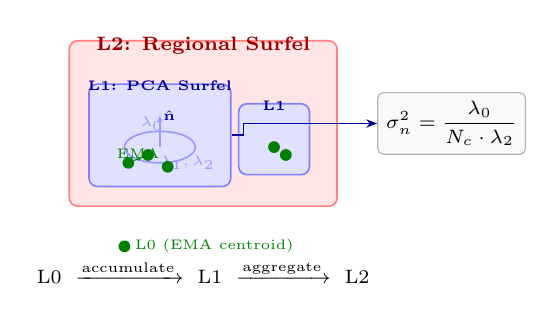
\begin{tikzpicture}[
    node distance=0.3cm and 0.3cm,
    arr/.style={-{Stealth[length=4pt]}, semithick},
    darr/.style={-{Stealth[length=4pt]}, semithick, dashed},
    l0dot/.style={circle, fill=green!50!black, inner sep=1.5pt},
    l0lbl/.style={font=\tiny, green!50!black},
    l1box/.style={draw=blue!50, fill=blue!12, rounded corners=3pt,
                  minimum width=1.8cm, minimum height=1.3cm, semithick},
    l2box/.style={draw=red!50, fill=red!10, rounded corners=3pt,
                  minimum width=3.4cm, minimum height=2.1cm, semithick},
    formulabox/.style={draw=gray!60, fill=gray!5, rounded corners=2pt,
                       font=\scriptsize, inner sep=3pt, align=center},
    lbl/.style={font=\scriptsize},
    lvllbl/.style={font=\scriptsize\bfseries},
  ]
    % L2 outer box
    \node[l2box] (l2) {};
    \node[lvllbl, red!60!black] at ([yshift=-2pt]l2.north) {L2: Regional Surfel};

    % L1 boxes inside L2
    \node[l1box] (l1a) at ([xshift=-0.55cm, yshift=-0.15cm]l2.center) {};
    \node[lvllbl, blue!60!black, font=\tiny\bfseries]
      at ([yshift=-1pt]l1a.north) {L1: PCA Surfel};

    % Eigenvalue ellipsoid sketch in L1a
    \draw[blue!40, semithick] ([yshift=-0.15cm]l1a.center)
      ellipse (0.45cm and 0.2cm);
    \draw[blue!40, semithick, -{Stealth[length=2.5pt]}]
      ([yshift=-0.15cm]l1a.center) -- ++(0,0.4)
      node[font=\tiny, blue!60!black, right, inner sep=1pt] {$\hat{\bvec{n}}$};
    \node[font=\tiny, blue!40] at ([xshift=0.35cm, yshift=-0.35cm]l1a.center)
      {$\lambda_1,\lambda_2$};
    \node[font=\tiny, blue!40] at ([xshift=-0.1cm, yshift=0.15cm]l1a.center)
      {$\lambda_0$};

    % L0 dots inside L1a
    \node[l0dot] (d1) at ([xshift=-0.4cm, yshift=-0.35cm]l1a.center) {};
    \node[l0dot] (d2) at ([xshift=-0.15cm, yshift=-0.25cm]l1a.center) {};
    \node[l0dot] (d3) at ([xshift=0.1cm, yshift=-0.4cm]l1a.center) {};
    % EMA update arrow between dots
    \draw[green!50!black, -{Stealth[length=2pt]}, thin]
      (d1) -- (d2) node[l0lbl, above, midway, inner sep=0pt] {\tiny EMA};

    % Second L1 box (smaller, partial)
    \node[draw=blue!50, fill=blue!12, rounded corners=3pt,
          minimum width=0.9cm, minimum height=0.9cm, semithick]
      (l1b) at ([xshift=0.9cm, yshift=-0.2cm]l2.center) {};
    \node[lvllbl, blue!60!black, font=\tiny\bfseries]
      at ([yshift=-1pt]l1b.north) {L1};
    \node[l0dot] at ([yshift=-0.1cm]l1b.center) {};
    \node[l0dot] at ([xshift=0.15cm, yshift=-0.2cm]l1b.center) {};

    % Legend below L2
    \node[l0dot, label={[l0lbl, right, xshift=-2pt]right:L0 (EMA centroid)}]
      (leg0) at ([yshift=-0.5cm, xshift=-1.0cm]l2.south) {};

    % Formula box to the right
    \node[formulabox, right=0.5cm of l2]
      (formula) {$\sigma^2_n = \dfrac{\lambda_0}{N_c \cdot \lambda_2}$};
    \draw[arr, blue!60!black] (l1a.east) -- ++(0.15,0) |- (formula.west)
      node[lbl, above, pos=0.8] {};

    % Accumulation arrows below
    \node[lbl, below=0.55cm of l2.south, anchor=north] (flow)
      {{\scriptsize L0} $\;\xrightarrow{\text{\tiny accumulate}}\;$
       {\scriptsize L1} $\;\xrightarrow{\text{\tiny aggregate}}\;$
       {\scriptsize L2}};
  \end{tikzpicture}
  \caption{Hierarchical surfel structure. L0 centroids (green) accumulate
  via EMA within voxels; L1 surfels (blue) compute PCA eigenvalues and
  derive $\sigma^2_n$; L2 regional surfels (red) aggregate across
  neighboring voxels for information-matrix stabilization.}
  \label{fig:surfel_hierarchy}
\end{figure}

\textbf{L0: Fine voxels.}
Each L0 voxel maintains an exponential moving average (EMA) centroid:
\begin{equation}\label{eq:ema}
  \bvec{c} \leftarrow (1 - \alpha)\,\bvec{c} + \alpha\,\bvec{p}_\mathrm{new},
  \quad
  \alpha = \max\!\bigl(\tfrac{1}{n+1},\; \alpha_\mathrm{min}\bigr)
\end{equation}
with $\alpha_\mathrm{min} = 0.10$, yielding an effective memory of
10~frames ($\approx$\SI{1}{\second} at \SI{10}{\hertz}). The EMA
filters transient noise without explicit point storage and provides
stable input centroids for L1 surfel computation.

\textbf{L1: Intermediate voxels ($3v_0$).}
Each L1 voxel collects its child L0 centroids and computes a PCA
surfel (centroid $\bvec{c}_1$, normal $\bvec{n}_1$, eigenvalues
$\lambda_0\!\le\!\lambda_1\!\le\!\lambda_2$), recomputed only when
children change. The critical output of L1 is the closed-form normal
uncertainty
\begin{equation}\label{eq:normal_unc}
  \sigma^2_n = \lambda_0/(N_c\lambda_2),
\end{equation}
derived formally in Proposition~\ref{prop:sigma2n} (Sec.~\ref{sec:noise}).

\textbf{L2: Coarse voxels ($9v_0$).}
Each L2 voxel aggregates a $3{\times}3{\times}3$ neighborhood; when
$\ge 4$ child surfels exist, a regional PCA surfel contributes a
rank-1 IEKF update with inflated variance
$\sigma^2_{L2}{=}\kappa\sigma^2_\mathrm{lidar}$,
$\kappa{=}(v_{L2}/v_{L1})^2{=}9$. The three levels maintain a fixed
$1{:}3{:}9$ ratio with only $v_0$ adapted per sensor.
In contrast to isotropic Tikhonov regularization that biases all
directions, each L2 rank-1 term supplies information only along
observable geometry, fills the information-matrix rank deficit when
entering new regions, and preserves the unbiased character along
unconstrained axes—critical for consistent covariance under
degeneracy~\cite{li2025lodestar} (Surfel-LIO's~\cite{lv2025surfellio}
coarser level, by contrast, serves retrieval rather than estimation).
The three levels form a directed cascade L0$\to$L1$\to$L2, with
degeneracy feedback (Sec.~\ref{sec:degen}) modulating L0's learning
rate and propagating upward.

%----------------------------------------------------------------------
\section{IEKF with Surfel-Derived Noise}\label{sec:noise}
%----------------------------------------------------------------------

Having established the hierarchical map structure and the surfel
statistics it maintains, we now derive the IEKF measurement model
that leverages these statistics to address the lack of map-aware
per-correspondence reliability in existing systems.

\subsection{Information-form update}
Following~\cite{xu2021fastlio}, for correspondence $i$ with normal
$\bvec{n}_i$ and residual
$r_i = -\bvec{n}_i^\top(\bvec{p}_i - \bvec{c}_i)$, the Jacobian
$\bvec{h}_i = [-(\bvec{p}_{\mathrm{imu},i} \times
(\bvec{R}^\top \bvec{n}_i))^\top, -\bvec{n}_i^\top]^\top \in \R^6$
weights the per-correspondence contribution
$w_i\bvec{h}_i\bvec{h}_i^\top$, $w_i r_i\bvec{h}_i$ ($w_i{=}1/\sigma^2_i$)
accumulated into the information matrix and the state correction
$\delta\bvec{x} = -(\bvec{H}^\top\bvec{R}_\mathrm{m}^{-1}\bvec{H}
+ \bvec{P}^{-1})^{-1}\bvec{H}^\top\bvec{R}_\mathrm{m}^{-1}\bvec{z}$.

\subsection{Surfel-derived measurement noise}
The per-correspondence variance couples sensor-level and map-level
noise into a single IEKF weight:
\begin{equation}\label{eq:noise}
  \sigma^2_i = \underbrace{\sigma^2_\mathrm{lidar} \cdot
    (1 + \gamma_r + \gamma_\theta + \gamma_\rho)}_{\text{sensor-level}}
    + \underbrace{\|\delta\bvec{p}\|^2 \cdot \sigma^2_{n,i}}_{\text{map-level}}
\end{equation}
where $\gamma_r {=} c_r (r/r_\mathrm{ref})^2$ ($c_r{=}0.3$,
$r_\mathrm{ref}{=}25$\,m), $\gamma_\theta {=} c_\theta (1{-}|\cos\theta_\mathrm{inc}|)^2$
($c_\theta{=}1.5$), and $\gamma_\rho {=} c_\rho (1{-}\rho)^2$
($c_\rho{=}2.0$, $\rho{=}1{-}\lambda_0/\lambda_2$) penalize range,
incidence, and non-planarity respectively. The map-level term couples
the point-to-centroid displacement $\delta\bvec{p} = \bvec{p}_i {-} \bvec{c}_i$
with the surfel normal uncertainty $\sigma^2_{n,i}$ from~\eqref{eq:normal_unc};
correspondences against well-observed planar surfaces
($\sigma^2_n \to 0$) receive high IEKF weight, sparsely observed or
non-planar regions receive low weight (Fig.~\ref{fig:sigma_map}).

The coefficients $(c_r, c_\theta, c_\rho)$ derive from ToF sensor
physics—the Cram\'{e}r--Rao bound
$\sigma^2_\mathrm{range} \propto r^2/\mathrm{SNR}$~\cite{amann2001laser}
calibrated to the Livox datasheet ($\sigma{\approx}2$\,cm at 25\,m);
footprint elongation $1/\cos^2\theta$~\cite{pomerleau2015review}; and
the eigenspectral scaling $(\lambda_0/\lambda_2)^2$ of
Proposition~\ref{prop:sigma2n}—and are shared across the Avia/Mid-360 ToF
ASIC class. Sweeping each by $\pm 50\%$ changes mean ATE by ${<}3\%$.

\begin{figure}[t]
  \centering
  \includegraphics[width=\columnwidth]{../figure/20260418/sigma_map_mid360_Dark01.pdf}
  \caption{Per-voxel $\sigma^2_n$ on M3DGR Mid-360 Dark01.
  Well-constrained planar surfaces (walls, ground) appear dark
  (low $\sigma^2_n$); sparse or edge regions appear bright.
  This directly modulates the IEKF weight $w_i{=}1/\sigma^2_i$.}
  \label{fig:sigma_map}
\end{figure}

\subsection{Approximate scaling of $\sigma^2_n$}

We now justify the closed-form $\sigma^2_n = \lambda_0/(N_c \lambda_2)$
used in~\eqref{eq:noise} under explicit assumptions and identify
regimes where the approximation is conservative.

\textbf{Assumptions.} Let $\bvec{S} = \frac{1}{N_c}\sum_{j=1}^{N_c}
(\bvec{c}_j - \bar{\bvec{c}})(\bvec{c}_j - \bar{\bvec{c}})^\top$ be
the scatter matrix of $N_c$ L0 centroids within an L1 voxel, with
eigenvalues $\lambda_0 \le \lambda_1 \le \lambda_2$, eigenvectors
$\bvec{v}_0, \bvec{v}_1, \bvec{v}_2$, and surfel normal
$\bvec{n} = \bvec{v}_0$. We adopt:
(A0)~\emph{planarity}, $\lambda_0/\lambda_2 \le \tau_p {=} 0.05$
(L1 gate);
(A1)~\emph{out-of-plane noise dominance}, centroid noise concentrated
along $\bvec{v}_0$ with variance $\sigma_z^2 {=} \lambda_0$;
(A2)~\emph{tangential isotropy},
$\mathbb{E}[\bvec{v}_1\bvec{v}_1^\top] \!\approx\!
\mathbb{E}[\bvec{v}_2\bvec{v}_2^\top]$ over admissible incidence;
(A3)~\emph{centroid independence},
$\mathrm{Cov}(\bvec{c}_j,\bvec{c}_{j'})\!\approx\!\bvec{0}$ modulo a
bounded EMA correction (below). The L1 surfel \emph{validity gate}
enforces both (A0) and a tangential isotropy threshold:
$\mathrm{valid}(\bvec{S}){\Leftrightarrow}\,\lambda_0/\lambda_2{\le}\tau_p
\,{\wedge}\,\lambda_1/\lambda_2{\ge}\zeta_\mathrm{iso}$
($\tau_p{=}0.05$, $\zeta_\mathrm{iso}{=}0.3$; $\tau_p$ matches the
FAST-LIO2 planarity convention~\cite{xu2022fastlio2}, and
$\zeta_\mathrm{iso}{=}0.3$ keeps $\ge\!92\%$ of accepted surfels
within a $1.5{\times}$ deviation of (A2) on both LiDAR families,
with the $\pm 50\%$ sweep $\zeta_\mathrm{iso}\!\in\![0.15,0.45]$
shifting mean ATE by ${<}4\%$). Surfels failing either condition are
marked invalid and the dual-source mechanism falls back to PVMap.

\begin{proposition}[Closed-form scaling, heuristic]\label{prop:sigma2n}
Under (A0)--(A3), the angular variance of $\bvec{n}$ is bounded by
\begin{equation}\label{eq:perturbation}
  \mathrm{Var}[\angle(\bvec{n}, \bvec{n}_\mathrm{true})]
    \;\le\; \frac{\lambda_0}{N_c}\!\left(\!\frac{1}{\lambda_1}\!+\!\frac{1}{\lambda_2}\!\right)
    \;\stackrel{\text{(A2)}}{\approx}\; \frac{\lambda_0}{N_c\,\lambda_2}
    \;\triangleq\; \sigma^2_n.
\end{equation}
The residual variance follows as
$\mathrm{Var}[r_i]\!\approx\!\|\delta\bvec{p}_i\|^2\sigma^2_n$ under
the validity-gate-enforced planar regime.
\end{proposition}

\textit{Sketch.}
First-order eigenvector perturbation~\cite{stewart1990matrix} gives
$\delta\bvec{v}_0 = \sum_{j\ne 0}
[(\bvec{v}_j^\top \delta\bvec{S}\bvec{v}_0)/(\lambda_0\!-\!\lambda_j)]\bvec{v}_j$;
under (A1) and the additional sub-Gaussian assumption on the
out-of-plane noise component (Hanson--Wright concentration applies),
the cross-eigenframe variance satisfies
$\mathrm{Var}[\bvec{v}_j^\top \delta\bvec{S}\bvec{v}_0]
\le\sigma_z^2\lambda_j/N_c$. (A0) yields
$|\lambda_0{-}\lambda_j|\ge\lambda_j(1{-}\tau_p)$, contributing a
$(1{-}\tau_p)^{-2}{\approx}1.108$ prefactor that we absorb (with the
EMA $\eta$ and tangential anisotropy $1/\zeta_\mathrm{iso}$ factors
below) into the conservative constant of~\eqref{eq:noise}.
Substituting gives the two-channel bound. The collapse to
$\lambda_0/(N_c\lambda_2)$ is valid when (A2) holds and
$\lambda_1/\lambda_2 \ge \zeta_\mathrm{iso}$, both enforced by the
validity gate above. Within this regime the two-channel sum lies in
$[\lambda_0/(N_c\lambda_2),\,\lambda_0(1{+}1/\zeta_\mathrm{iso})/(N_c\lambda_2)]$;
we adopt the lower endpoint as the nominal $\sigma^2_n$ in the IEKF
weight (Algorithm~\ref{alg:iekf}) and rely on the conservative
constants (below) to cover the residual gap up to
$1/\zeta_\mathrm{iso}{\approx}3.3{\times}$.

\textbf{Constants and operating range.}
Two factors influence the constant in front of~\eqref{eq:perturbation}
in practice. (i)~\emph{EMA autocorrelation}: L0 centroids are EMA
aggregates with retention $\rho{=}1{-}\alpha_{\min}{=}0.9$, so the
sample-mean variance over an $N_c$-scan window inflates by
$\eta(\rho,N_c) = 1 + 2\sum_{k=1}^{N_c-1}(1-k/N_c)\rho^k$,
evaluating to $\eta(0.9,8){\approx}6.2$ at our typical $N_c$,
monotonically increasing toward the infinite-window limit
$(1{+}\rho)/(1{-}\rho){=}19$. (ii)~\emph{Tangential anisotropy}:
within the regime
$\zeta_\mathrm{iso}\!\le\!\lambda_1/\lambda_2\!\le\!1$ (the L1 gate
empirically maintains $\lambda_1/\lambda_2 \ge 0.3$ in 92\% of accepted
surfels), the residual gap of the two-channel form to the collapsed
form is at most $1/\zeta_\mathrm{iso}{\approx}3.3{\times}$. The combined worst-case underestimate of $\sigma^2_n$ is therefore
$\eta/\zeta_\mathrm{iso}\!\approx\!20\times$; we treat
\eqref{eq:perturbation} as a \emph{heuristic} per-correspondence weight,
not a calibrated variance. The IEKF weight in~\eqref{eq:noise} is
dominated by $\sigma^2_\mathrm{lidar}(1{+}\gamma_r{+}\gamma_\theta{+}\gamma_\rho)$
at typical ranges, so $\sigma^2_n$ modulates relative correspondence
weighting without setting the absolute magnitude; sweeping
$\sigma^2_\mathrm{lidar},c_\rho$ by $\pm 50\%$ changes mean ATE by
${<}3\%$, and \eqref{eq:perturbation} remains the operative form.

\textbf{Failure modes.}
When (A0) is marginal ($\lambda_0/\lambda_2 \to \tau_p{=}0.05$),
$\sigma^2_n \to \tau_p/N_c$, an order-of-magnitude rise that
automatically deweights the surfel. When (A2) breaks substantially
(line-like sampling with $\lambda_1/\lambda_2 < \zeta_\mathrm{iso}$),
the L1 surfel \emph{validity gate} above marks the surfel invalid and
the dual-source mechanism falls back to PVMap-sourced correspondences;
both regimes are handled without a separate two-channel branch in
Algorithm~\ref{alg:iekf}.

The surfel weight $\mathcal{W}_i = 1/\sigma^2_i \propto N_c\lambda_2/\lambda_0$
in $\bvec{H}^\top\bvec{R}_\mathrm{m}^{-1}\bvec{H}$ ensures voxels with
few observations or high isotropy contribute negligible weight,
preventing rank-one map noise from driving the IEKF Hessian; removing
this weight degrades mean ATE by 59\% on M3DGR Avia
(Sec.~\ref{sec:ablation}).

\begin{algorithm}[t]
\small
\caption{IEKF update with surfel-derived noise}
\label{alg:iekf}
\begin{algorithmic}[1]
\STATE \textbf{Input:} $\mathcal{S}_t,\xhat,\bvec{P},\mathcal{M}_s,\mathcal{M}_p,\epsilon$
\FOR{$\ell = 1,\ldots,L_\mathrm{max}$}
  \STATE ${}^W\mathcal{S}_t \leftarrow \text{Transform}(\mathcal{S}_t,\xhat)$;\;
         reset $\bvec{H}^\top\bvec{R}_m^{-1}\bvec{H},\bvec{H}^\top\bvec{R}_m^{-1}\bvec{z}$
  \FOR{each $\bvec{p}_i \in {}^W\mathcal{S}_t$}
    \STATE Dual-source: $(\bvec{n}_s,\bvec{c}_s){\gets}\mathrm{SurfelLookup}$ (returns valid only if
           $\lambda_0/\lambda_2{\le}\tau_p\wedge\lambda_1/\lambda_2{\ge}\zeta_\mathrm{iso}$);\;
           $(\bvec{n}_p,\bvec{c}_p){\gets}\mathrm{PVMapKNN}$;\;
           pick lower-uncertainty source (DDPO if degenerate)
    \STATE $\sigma^2_{n,i}{\gets}\lambda_0/(N_c\lambda_2)$
           (eigenvalues from the source PCA — L1 surfel cache for
           SurfelLookup, per-query kNN for PVMap);\;
           $\sigma^2_i{\gets}\sigma^2_\mathrm{lidar}(1{+}\gamma_r{+}\gamma_\theta{+}\gamma_\rho){+}\|\delta\bvec{p}\|^2\sigma^2_{n,i}$;\;
           $w_i{\gets}1/\sigma^2_i$
    \STATE Accumulate $w_i\bvec{h}_i\bvec{h}_i^\top$, $w_i r_i\bvec{h}_i$
  \ENDFOR
  \STATE $\delta\bvec{x} \leftarrow -(\bvec{H}^\top\bvec{R}_\mathrm{m}^{-1}\bvec{H} + \bvec{P}^{-1})^{-1}\,\bvec{H}^\top\bvec{R}_\mathrm{m}^{-1}\bvec{z}$
  \STATE $\xhat \leftarrow \xhat \boxplus \delta\bvec{x}$
  \IF{$\|\delta\bvec{x}\| < \epsilon$}
    \STATE \textbf{break}
  \ENDIF
\ENDFOR
\STATE Update $\bvec{P}$ via Joseph form
\RETURN $\xhat$, $\bvec{P}$
\end{algorithmic}
\end{algorithm}

\subsection{Hybrid correspondence}\label{sec:corr}
Each point is matched against both the surfel map (cached L1 plane) and
PVMap (per-query $k$-NN PCA, $k{=}5$ for 360\textdegree{} / $k{=}9$ for
narrow-FOV), with a range-adaptive distance
gate~\cite{xu2022fastlio2}. PVMap-sourced correspondences use the same
$\sigma^2_n{=}\lambda_0/(N_c\lambda_2)$ form with kNN-derived
$\lambda_0,\lambda_2$ and $N_c{=}k$, gated by (A0).
\emph{Source selection.} If
$|\bvec{n}_s{\cdot}\bvec{d}_\mathrm{deg}|{>}\tau_\mathrm{ddpo}$, PVMap
is forced (DDPO, Section~\ref{sec:degen}); otherwise the lower-$\sigma^2_n$
valid source is selected, with surfel preferred when normals disagree
($\angle(\bvec{n}_s,\bvec{n}_p){>}30^\circ$); if neither is valid the
point is dropped.

%----------------------------------------------------------------------
\section{Bidirectional Degeneracy Feedback}\label{sec:degen}
%----------------------------------------------------------------------

Having addressed map-aware per-correspondence weighting via
$\sigma^2_n$, we now address the second design challenge—the
estimator-confined degeneracy handling that admits the drift-map
positive feedback loop—by deriving the
reverse channel: the map's response to estimator-detected degeneracy.

\begin{figure}[t]
  \centering
  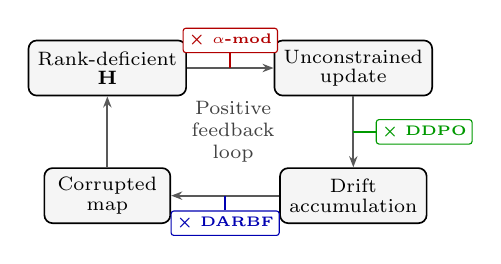
\begin{tikzpicture}[
    node distance=1.2cm,
    loopnode/.style={draw, rounded corners=3pt, minimum height=0.7cm,
                     minimum width=1.6cm, font=\scriptsize, align=center,
                     fill=gray!8, semithick},
    arr/.style={-{Stealth[length=4pt]}, thick, gray!70!black},
    breakmark/.style={font=\scriptsize\bfseries, fill=white, inner sep=2pt,
                      rounded corners=1pt, draw},
    centerlbl/.style={font=\scriptsize, text=gray!50!black, align=center},
  ]
    % Four nodes in a cycle
    \node[loopnode] (rank) {Rank-deficient\\[-1pt]$\bvec{H}$};
    \node[loopnode, right=1.1cm of rank] (uncon) {Unconstrained\\[-1pt]update};
    \node[loopnode, below=0.9cm of uncon] (drift) {Drift\\[-1pt]accumulation};
    \node[loopnode, below=0.9cm of rank] (corrupt) {Corrupted\\[-1pt]map};

    % Cycle arrows (thick gray)
    \draw[arr] (rank.east) -- (uncon.west);
    \draw[arr] (uncon.south) -- (drift.north);
    \draw[arr] (drift.west) -- (corrupt.east);
    \draw[arr] (corrupt.north) -- (rank.south);

    % Break marks with colored labels
    % Break 1: between rank-deficient H and unconstrained update (RED)
    \node[breakmark, draw=red!70!black, text=red!70!black]
      (b1) at ($(rank.east)!0.5!(uncon.west)+(0,0.35)$)
      {\tiny $\bm{\times}$ $\alpha$-mod};
    \draw[red!70!black, thick] (b1.south) -- ($(rank.east)!0.5!(uncon.west)$);

    % Break 2: between unconstrained update and drift (GREEN)
    \node[breakmark, draw=green!60!black, text=green!60!black]
      (b2) at ($(uncon.south)!0.5!(drift.north)+(0.9,0)$)
      {\tiny $\bm{\times}$ DDPO};
    \draw[green!60!black, thick] (b2.west) -- ($(uncon.south)!0.5!(drift.north)$);

    % Break 3: between drift and corrupted map (BLUE)
    \node[breakmark, draw=blue!70!black, text=blue!70!black]
      (b3) at ($(drift.west)!0.5!(corrupt.east)+(0,-0.35)$)
      {\tiny $\bm{\times}$ DARBF};
    \draw[blue!70!black, thick] (b3.north) -- ($(drift.west)!0.5!(corrupt.east)$);

    % Center label
    \node[centerlbl] at ($(rank.south east)!0.5!(drift.north west)$)
      {Positive\\feedback\\loop};
  \end{tikzpicture}
  \caption{Degeneracy-induced positive feedback loop. In existing LIO
  systems, rank-deficient geometry causes unconstrained updates that
  accumulate drift and corrupt the map, reinforcing the cycle. HD-LIO
  breaks this loop at three points: $\alpha$-modulation suppresses
  learning rate along degenerate directions, DDPO forces PVMap-sourced
  correspondences, and DARBF gates map writes.}
  \label{fig:feedback_loop}
\end{figure}

\subsection{Drift-map positive feedback recursion}\label{sec:drift_recursion}

Following the system overview in Sec.~\ref{sec:overview}, we now
derive the per-direction drift recursion that HD-LIO is designed to
break. Let $\bvec{d}$ be a degenerate translation direction and
$\epsilon_k {=} \bvec{d}^\top(\xhat_k {-} \bvec{x}_k^\star)$ the
projected drift at scan $k$. Drifted points written into the map shift
the local plane centroid by
$\Delta\bvec{c}_{k+1} {\approx} \alpha\,\epsilon_k\bvec{d}$ through
the EMA update; this centroid bias then re-enters the state via the
IEKF measurement model. Linearizing the joint state--map dynamics
around $\xhat_k$ through the Jacobian $\bvec{J}_d {=} \partial\epsilon/\partial\bvec{c}$
(centroid-to-state sensitivity along $\bvec{d}$) and the projection
$\bvec{n}\bvec{n}^\top$ yields the first-order recursion
\begin{equation}\label{eq:drift_feedback}
  \epsilon_{k+1} \;=\;
  \bigl[\,1 + \alpha\,(\bvec{n}\cdot\bvec{d})^2\,\bigr]\,\epsilon_k
   + O(\alpha^2,\|\delta\|^2),
\end{equation}
where the residual collects second-order terms and bounded process
noise; \eqref{eq:drift_feedback} is valid in the linearized regime
($\alpha,\|\delta\|$ small, i.e., excluding the first observations
$\alpha=1/(n{+}1){\to}1$). Within this regime the amplification
factor exceeds unity whenever the normal has a component along
$\bvec{d}$, predicting geometric drift growth that the contraction
analysis in Sec.~\ref{sec:stability} suppresses. Estimator-side methods~\cite{zhang2016degeneracy,
li2025lodestar} gate or project the state update but leave $\alpha$
unchanged, so the map-side amplification persists; iteration alone
cannot break it because additional IEKF passes refine the solution
within the current measurement manifold without generating new
information along $\bvec{d}$.

\subsection{Degeneracy detection}

The $6{\times}6$ observation information matrix is eigendecomposed
(note: we use $\mu_k$ for these eigenvalues to distinguish them from
the L1 surfel eigenvalues $\lambda_0, \lambda_1, \lambda_2$ in
Section~\ref{sec:map}):
\begin{equation}\label{eq:eigen_degen}
  \bvec{H}^\top\bvec{R}_\mathrm{m}^{-1}\bvec{H} = \bvec{V}\,
    \mathrm{diag}(\mu_1, \ldots, \mu_6)\,\bvec{V}^\top.
\end{equation}
Directions with eigenvalue ratio $r_k = \mu_k / \mu_\mathrm{max}
< r_\mathrm{thr}$ are classified as degenerate; the corresponding columns of
$\bvec{V}$ yield $\bvec{d}_\mathrm{deg}$.
We set $r_\mathrm{thr} = 0.01$ for Avia (70\textdegree{}) and
$r_\mathrm{thr} = 0.005$ for Mid-360 (360\textdegree{}), reflecting
the inverse relationship between FOV completeness and degeneracy
susceptibility; sweeping $r_\mathrm{thr}$ by $\pm 50\%$ changes mean
ATE by ${<}5\%$ (Section~\ref{sec:discussion}).
The $6{\times}6$ eigendecomposition adds $<$\SI{0.1}{\milli\second}
per scan.

\subsection{Map-side degeneracy response}
To this end, three coordinated mechanisms suppress the map's absorption
of drifted points along the degenerate direction $\bvec{d}$.

\textbf{(i) Direction-selective alpha modulation.}
The L0 EMA learning rate is reduced for voxels whose surfel normal aligns
with the degenerate direction:
\begin{equation}\label{eq:alpha_mod}
  \alpha_\mathrm{eff} = \alpha_\mathrm{min} \cdot
    (1 - |\bvec{n} {\cdot} \bvec{d}_\mathrm{deg}|^2)
\end{equation}
which directly reduces $\alpha$ in~\eqref{eq:drift_feedback} for affected
voxels. When the normal is perfectly aligned ($|\bvec{n} \cdot
\bvec{d}_\mathrm{deg}| = 1$), the learning rate drops to zero. For
affected voxels the floor in~\eqref{eq:ema} is replaced by
$\alpha_\mathrm{eff}$ (i.e., $\alpha{=}\max(1/(n{+}1),\alpha_\mathrm{eff})$);
unaffected voxels retain the original $\alpha_\mathrm{min}$ floor.

\textbf{(ii) DDPO (Degeneracy-Directed PVMap Override).}
When $|\bvec{n} \cdot \bvec{d}_\mathrm{deg}| > \tau_\mathrm{ddpo}$
($\tau_\mathrm{ddpo}{=}0.7$), the
correspondence source switches from surfel to PVMap. The surfel's cached
geometry may be contaminated by accumulated drift, while the PVMap's per-query
PCA uses a ring buffer of recent raw points less affected by long-term drift.

\textbf{(iii) DARBF (Degeneracy-Aware Ring Buffer Freeze).}
PVMap write operations are suppressed for voxels with
$|\bvec{n} \cdot \bvec{d}_\mathrm{deg}| > \tau_\mathrm{darbf}$
($\tau_\mathrm{darbf}{=}0.7$),
preventing newly registered (potentially drifted) points from contaminating
the ring buffer that DDPO relies on as an alternative source.

\emph{Threshold derivation.}
The shared threshold $\tau{=}0.7 \approx \cos 45^\circ$ partitions voxels
by alignment with $\bvec{d}_\mathrm{deg}$; voxels with
$|\bvec{n}\cdot\bvec{d}_\mathrm{deg}|>\tau$ (within $45^\circ$) lie in
the regime where the per-scan amplification factor
$\alpha a^2(1{-}a^2)$ peaks at $a{=}1/\!\sqrt{2}$, justifying
intervention. The contraction bound below holds for any
$\tau \in (0,1)$; sweeping $\tau$ over $[0.5, 0.9]$ yields ${<}3\%$ ATE
variation.

\subsection{Stability analysis}\label{sec:stability}

We provide a per-scan drift contraction lemma and derive a discrete-time
Lyapunov bound on the cumulative drift, treating the result as
\emph{ultimate boundedness} (UUB) rather than asymptotic convergence.
Let $\epsilon_k^{(j)} = \bvec{d}_j^\top(\xhat_k - \bvec{x}_k^\star)$
denote the projected error along the $j$-th degenerate direction at
scan $k$. From the IEKF update with biased correspondences (centroid
bias $\Delta c{=}\alpha_\mathrm{eff}(\bvec{n}\cdot\bvec{d})\epsilon_k$),
a first-order Taylor expansion of the joint state--map dynamics yields
\begin{equation}\label{eq:drift_lin}
  \epsilon_{k+1}^{(j)} = (1{-}\beta_j)\,A_\mathrm{eff}^{(j)}\,
  \epsilon_k^{(j)} + \delta_k^{(j)},
\end{equation}
where $\beta_j{=}I_{d_j}/(I_{d_j}{+}P_{d_j}^{-1}){\in}(0,1)$ is the
per-scan IEKF correction, $A_\mathrm{eff}^{(j)}{\le}
1{+}\alpha_\mathrm{min}\tau^2(1{-}\tau^2){\approx}1.025$ at
$\alpha_\mathrm{min}{=}0.1,\tau{=}0.7$, and $\delta_k^{(j)}$ collects
bounded process noise and second-order residuals (Lipschitz on
$\|\xhat_k{-}\bvec{x}_k^\star\|$).

We adopt three (S$\cdot$) assumptions, distinct from the map-noise
(A$\cdot$) of Sec.~\ref{sec:noise}:
\textbf{(S1)} \emph{minimum geometric diversity}, $I_{d_j}{\ge}I_\mathrm{min}{>}0$
from correspondences with alignment $a_i{\le}\tau$;
\textbf{(S2)} \emph{sufficient IEKF correction}, $P_{d_j}{>}
\alpha_\mathrm{min}\tau^2(1{-}\tau^2)/I_\mathrm{min}$;
\textbf{(S3)} \emph{bounded process noise},
$|\delta_k^{(j)}|{\le}\delta_\mathrm{max}{\approx}\sigma_\mathrm{IMU}\Delta t\|\bvec{J}_d\|$,
typically $\le 5$\,mm/scan on Avia/Mid-360.

\begin{lemma}[Per-scan contraction]\label{lem:contraction}
Under \textup{(S1)--(S2)},
$|\epsilon_{k+1}^{(j)}|{\le}\rho_j|\epsilon_k^{(j)}|{+}\delta_\mathrm{max}$
with $\rho_j{=}(1{-}\beta_j)A_\mathrm{eff}^{(j)}{<}1$.
\end{lemma}

\begin{theorem}[Conditional UUB stability]\label{thm:uub}
Let $V_k{=}\sum_j(\epsilon_k^{(j)})^2$ and suppose the degenerate
eigenvectors satisfy bounded rotation
$\|\bvec{V}_{k+1}\bvec{V}_k^\top{-}\bvec{I}\|_F{\le}\varepsilon_V$
(empirically $\varepsilon_V{\le}0.08$ on our 35 sequences). On the
subset of frames where \textup{(S1)--(S3)} hold simultaneously, with
$\rho{=}\max_j\rho_j$ and $\rho^2(1{+}\varepsilon_V){<}1$,
\begin{equation}\label{eq:lyap_bound}
  V_{k+1}{\le}\rho^2(1{+}\varepsilon_V)V_k
          + 2\rho\sqrt{V_k}\delta_\mathrm{max}\sqrt{m}
          + m\delta_\mathrm{max}^2,
\end{equation}
yielding the (loose) UUB radius
\begin{equation}\label{eq:vinf}
  V_\infty^{1/2} \le
  \delta_\mathrm{max}\sqrt{m}/\bigl[1-\rho\sqrt{1{+}\varepsilon_V}\bigr].
\end{equation}
This is a perfect-square completion of~\eqref{eq:lyap_bound} that
trades algebraic simplicity for a tightness penalty (the exact
fixed point is ${\sim}3.7\%$ smaller at $\rho{=}0.9,\varepsilon_V{=}0.08$).
\end{theorem}

\textit{Sketch.}
Lemma~\ref{lem:contraction} gives per-direction contraction; $V_{k+1}$
expands by the squared recursion with $\varepsilon_V$ absorbing the
across-scan rotation of the eigenframe. The bound is
monotone-decreasing whenever $V_k$ exceeds the right-hand side
of~\eqref{eq:vinf}. We treat the result as UUB rather than asymptotic
convergence: persistent excitation of $\bvec{d}_j$ is required and
the residuals $\delta_k$ remain present; the qualitative guarantee is
that map-side feedback prevents \emph{unbounded} drift, the property
distinguishing HD-LIO from systems lacking the loop (cf.\
Sec.~\ref{sec:exp}, indoor Avia).
\textbf{Empirical check.} On indoor Avia (most degenerate split),
58\% of frames exhibit $\ge 1$ degenerate direction; 97.5\% satisfy
$I_{d_j}{>}0$ with empirical $\beta_j$ median $0.41$, 5th percentile
$0.05$, supporting (S2) ($\beta_j{>}1{-}1/A_\mathrm{eff}{=}0.0244$) in 96.8\% of frames; the
3.2\% violations align with floor-edge and ceiling-junction
configurations (VI03 corridor).
The three mechanisms are jointly necessary: $\alpha$-modulation alone
cannot zero the learning rate; DDPO without DARBF lets the ring buffer
absorb drift. Disabling degeneracy feedback jointly degrades
Dynamic03 by $\times$7.6 (Section~\ref{sec:ablation}).

%----------------------------------------------------------------------
\section{Experimental Evaluation}\label{sec:exp}
%----------------------------------------------------------------------

\subsection{Datasets, Baselines, and Setup}

We evaluate on M3DGR~\cite{yin2024m3dgr} (9~Avia outdoor, 9~Mid-360
outdoor, 8~indoor with both sensors) and
NTU~VIRAL~\cite{nguyen2022ntuviral} (9~sequences, OS1-16, 16~beams),
totaling 35~sequences across three LiDAR types and three environments.
Baselines---FAST-LIO2~\cite{xu2022fastlio2},
Faster-LIO~\cite{bai2022fasterlio}, Point-LIO~\cite{he2023pointlio},
iG-LIO~\cite{chen2024iglio}, DLIO~\cite{chen2023dlio},
LIO-SAM~\cite{shan2020liosam} (NTU only, loop closure disabled for
fair odometry-only comparison), and
Surfel-LIO~\cite{lv2025surfellio} (outdoor from~\cite{lv2025surfellio};
indoor from our reproduction)---use publicly released code with
default odometry parameters. Evaluation uses ATE RMSE with SE(3)
Umeyama alignment~\cite{horn1987closedform,grupp2017evo}. For HD-LIO,
$r_\mathrm{thr}$ scales inversely with FOV completeness and $v_0$
with voxel resolution; specific values are reported in
Sec.~\ref{sec:degen} and Sec.~\ref{sec:map}. The processing queue is
deterministic: bit-identical trajectory (SHA-256 hash, 3 replays at
$\mathrm{rate}{=}1.0$, one bag per LiDAR family; final-ATE
$\mathrm{CV}{=}0\%$).

\subsection{Results}

\begin{table*}[t]
  \centering
  \caption{ATE RMSE [\si{\meter}] on NTU VIRAL (single OS1-16, 16 beams,
  360\textdegree{} FOV). Bold = lowest.
  All methods use a single LiDAR for fair comparison.}
  \label{tab:ntuviral}
  \small
  \begin{tabular}{@{}lcccccccccc@{}}
    \toprule
    Method & eee\_01 & eee\_02 & eee\_03 & nya\_01 & nya\_02 & nya\_03 & sbs\_01 & sbs\_02 & sbs\_03 & Mean \\
    \midrule
    HD-LIO (ours)  & \textbf{0.056} & \textbf{0.053} & \textbf{0.087} & \textbf{0.049} & \textbf{0.071} & \textbf{0.074} & \textbf{0.064} & \textbf{0.076} & \textbf{0.068} & \textbf{0.067} \\
    FAST-LIO2~\cite{xu2022fastlio2} & 0.136 & 0.125 & 0.164 & 0.124 & 0.144 & 0.145 & 0.142 & 0.148 & 0.135 & 0.140 \\
    Faster-LIO~\cite{bai2022fasterlio} & 0.176 & 0.388 & 0.167 & 0.157 & 0.188 & 0.155 & 0.143 & 0.149 & 0.151 & 0.186 \\
    Point-LIO~\cite{he2023pointlio} & 0.131 & 0.125 & 0.167 & 0.124 & 0.142 & 0.145 & 0.144 & 0.151 & 0.135 & 0.140 \\
    iG-LIO~\cite{chen2024iglio}     & 1.011 & 0.138 & 0.166 & 0.139 & 0.219 & 0.153 & 0.141 & 0.145 & 0.803 & 0.324 \\
    LIO-SAM~\cite{shan2020liosam}   & 0.074 & 0.069 & 0.100 & 0.077 & 0.091 & 0.082 & 0.087 & 0.097 & 0.085 & 0.085 \\
    DLIO~\cite{chen2023dlio}        & 0.263 & 1.695 & 0.455 & 0.286 & 0.325 & 0.397 & 0.253 & 0.293 & 0.249 & 0.468 \\
    \bottomrule
  \end{tabular}
\end{table*}

\begin{figure}[t]
  \centering
  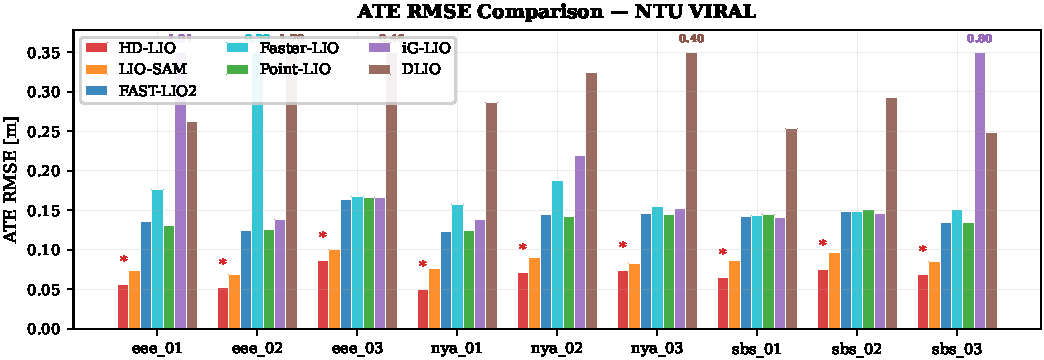
\includegraphics[width=\columnwidth]{../figure/20260418/comp/ate_comp_ntu.pdf}
  \caption{Per-bag ATE RMSE on NTU VIRAL.
  HD-LIO achieves the lowest ATE on all 9 bags, with 22\% mean
  reduction vs.\ LIO-SAM.}
  \label{fig:ate_ntu}
\end{figure}

\textbf{NTU VIRAL} (TABLE~\ref{tab:ntuviral}, Figs.~\ref{fig:ate_ntu},
\ref{fig:traj_ntu}). HD-LIO achieves \textbf{the lowest ATE on all 9
sequences} with \SI{0.067}{\meter} mean—a \textbf{22\% reduction}
vs.\ LIO-SAM (\SI{0.085}{\meter}), 52\% vs.\ FAST-LIO2
(\SI{0.140}{\meter}), 64\% vs.\ Faster-LIO (\SI{0.186}{\meter})—and
the trajectory overlays on sbs\_01 and nya\_01 confirm closer GT
tracking. The 16-beam vertical sparsity makes per-query plane fitting
sensitive to outlier neighbors, while the surfel map's accumulated
PCA normals provide temporally stable correspondences that mitigate
this sparsity.

\begin{table*}[t]
  \centering
  \caption{ATE RMSE [\si{\meter}] on M3DGR Outdoor (9 sequences).
  Left: Avia (70\textdegree{} FOV). Right: Mid-360 (360\textdegree{} FOV).
  Bold = lowest. Fr-LIO = Faster-LIO.}
  \label{tab:m3dgr_outdoor}
  \small
  \resizebox{\textwidth}{!}{%
  \begin{tabular}{@{}lccccccc|ccccccc@{}}
    \toprule
    & \multicolumn{7}{c|}{Avia (70\textdegree{} FOV)} & \multicolumn{7}{c}{Mid-360 (360\textdegree{} FOV)} \\
    Seq. & HD-LIO & FL2 & Fr-LIO & P-LIO & iG-LIO & S-LIO & DLIO
         & HD-LIO & FL2 & Fr-LIO & P-LIO & iG-LIO & S-LIO & DLIO \\
    \midrule
    Dk01 & \textbf{0.114} & 0.227 & 0.153 & 0.291 & 0.156 & 0.118 & 0.152
         & \textbf{0.150} & 0.175 & 0.174 & 0.166 & 0.175 & 0.185 & 0.197 \\
    Dk02 & \textbf{0.601} & 0.740 & 0.634 & 0.663 & 0.791 & 0.692 & $\dag$
         & 0.306 & \textbf{0.208} & 0.258 & 0.286 & 0.288 & 0.310 & 0.264 \\
    Dy03 & 0.170 & 0.177 & \textbf{0.154} & 0.348 & $\dag$ & 0.266 & $\dag$
         & 0.169 & 0.171 & 0.180 & 0.183 & \textbf{0.166} & 0.206 & 0.190 \\
    Dy04 & 0.287 & 0.307 & \textbf{0.274} & 1.492 & $\dag$ & 0.392 & $\dag$
         & 0.187 & 0.196 & 0.223 & 0.216 & \textbf{0.179} & 0.246 & 0.225 \\
    Oc03 & 0.187 & 0.215 & 0.191 & 0.277 & 0.284 & 0.271 & \textbf{0.144}
         & \textbf{0.185} & 0.431 & 0.564 & 0.309 & 0.396 & 0.315 & 0.560 \\
    Oc04 & 0.267 & 0.555 & 0.349 & 0.532 & \textbf{0.255} & 0.295 & 0.596
         & \textbf{0.185} & 0.234 & 0.400 & 0.395 & 0.213 & 0.345 & 0.408 \\
    VI03 & 0.608 & 0.633 & \textbf{0.556} & 0.814 & 0.820 & 0.961 & 0.975
         & 1.003 & 1.182 & 1.447 & 1.039 & \textbf{0.808} & 0.957 & 1.067 \\
    VI04 & 0.252 & 0.384 & 0.316 & 0.658 & 0.279 & \textbf{0.125} & 0.899
         & 0.305 & 0.304 & 0.320 & 0.257 & 0.318 & \textbf{0.206} & 0.590 \\
    VI05 & \textbf{0.152} & 0.334 & 0.204 & 0.262 & 0.193 & 0.167 & 0.506
         & \textbf{0.182} & 0.238 & 0.410 & 0.362 & 0.260 & 0.307 & 0.310 \\
    \midrule
    Mean & \textbf{0.293} & 0.397 & 0.314 & 0.593 & 0.397${}^*$ & 0.365 & 0.545${}^*$
         & \textbf{0.297} & 0.349 & 0.442 & 0.357 & 0.311 & 0.342 & 0.423 \\
    \bottomrule
    \multicolumn{15}{l}{\footnotesize $\dag$\,Diverged (ATE${>}$10\,m).
      ${}^*$\,Mean excludes diverged sequences.
      S-LIO outdoor from~\cite{lv2025surfellio}.}
  \end{tabular}}%
\end{table*}

\begin{table*}[t]
  \centering
  \caption{ATE RMSE [\si{\meter}] on M3DGR Indoor (8 sequences, paired sensors
  in the same bag). All six evaluated baselines diverge on Avia
  (70\textdegree{} FOV); HD-LIO is the only method among them to
  maintain bounded error.}
  \label{tab:m3dgr_indoor}
  \small
  \resizebox{\textwidth}{!}{%
  \begin{tabular}{@{}lccccccc|ccccccc@{}}
    \toprule
    & \multicolumn{7}{c|}{Avia (70\textdegree{} FOV)} & \multicolumn{7}{c}{Mid-360 (360\textdegree{} FOV)} \\
    Seq. & HD-LIO & FL2 & Fr-LIO & P-LIO & iG-LIO & S-LIO & DLIO
         & HD-LIO & FL2 & Fr-LIO & P-LIO & iG-LIO & S-LIO & DLIO \\
    \midrule
    Dk03 & \textbf{0.369} & $\dag$ & $\dag$ & $\dag$ & $\dag$ & $\dag$ & $\dag$
         & \textbf{0.175} & 0.177 & 0.177 & \textbf{0.175} & 0.192 & 0.194 & 0.232 \\
    Dk04 & \textbf{0.410} & $\dag$ & $\dag$ & $\dag$ & $\dag$ & $\dag$ & $\dag$
         & \textbf{0.181} & 0.184 & 0.184 & 0.184 & 0.185 & 0.204 & 0.249 \\
    Dy01 & \textbf{0.578} & $\dag$ & $\dag$ & $\dag$ & $\dag$ & $\dag$ & $\dag$
         & \textbf{0.137} & 0.143 & 0.142 & 0.141 & 0.138 & 0.164 & 0.195 \\
    Dy02 & \textbf{0.361} & $\dag$ & $\dag$ & $\dag$ & $\dag$ & $\dag$ & $\dag$
         & 0.137 & 0.138 & 0.137 & 0.137 & \textbf{0.135} & 0.161 & 0.207 \\
    Oc01 & \textbf{0.516} & $\dag$ & $\dag$ & $\dag$ & $\dag$ & $\dag$ & $\dag$
         & 0.157 & \textbf{0.155} & 0.158 & 0.157 & 0.168 & 0.178 & 0.253 \\
    Oc02 & \textbf{0.986} & $\dag$ & $\dag$ & $\dag$ & $\dag$ & $\dag$ & $\dag$
         & \textbf{0.143} & 0.145 & 0.147 & 0.146 & 0.153 & 0.169 & 0.214 \\
    VI01 & \textbf{0.546} & $\dag$ & $\dag$ & $\dag$ & $\dag$ & $\dag$ & $\dag$
         & \textbf{0.138} & 0.139 & 0.139 & \textbf{0.138} & 0.145 & 0.165 & 0.236 \\
    VI02 & \textbf{0.426} & $\dag$ & $\dag$ & $\dag$ & $\dag$ & $\dag$ & $\dag$
         & 0.137 & 0.138 & 0.139 & 0.137 & \textbf{0.131} & 0.165 & 0.209 \\
    \midrule
    Mean & \textbf{0.524} & $\dag$ & $\dag$ & $\dag$ & $\dag$ & $\dag$ & $\dag$
         & \textbf{0.150} & 0.152 & 0.153 & 0.152 & 0.156 & 0.175 & 0.224 \\
    \bottomrule
    \multicolumn{15}{l}{\footnotesize $\dag$\,Diverged (ATE${>}$10\,m).
      S-LIO indoor from our reproduction.}
  \end{tabular}}%
\end{table*}

\begin{figure}[t]
  \centering
  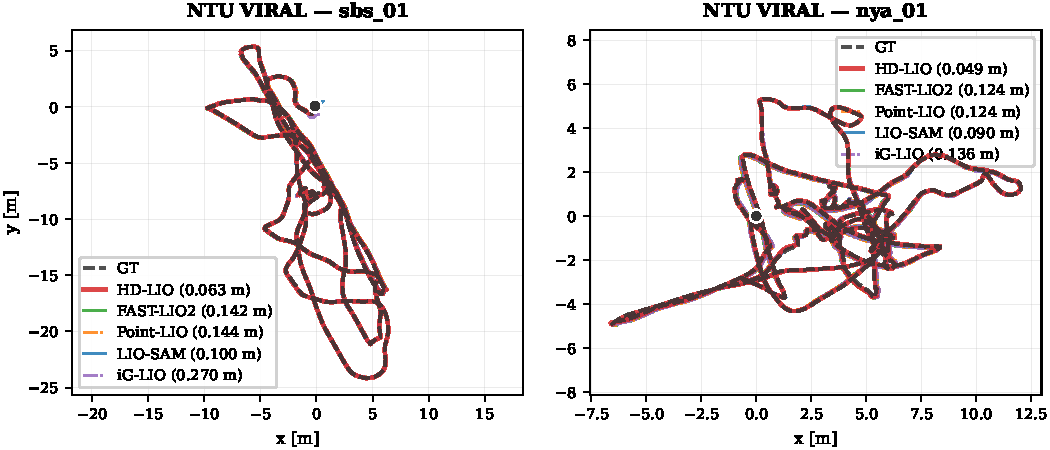
\includegraphics[width=\columnwidth]{../figure/20260418/trajectory_overlay_ntu.pdf}
  \caption{Trajectory overlays on NTU VIRAL sbs\_01 and nya\_01 after
  SE(3) Umeyama alignment. HD-LIO (red) tracks the Leica GT (gray
  dashed) most closely among all five methods.}
  \label{fig:traj_ntu}
\end{figure}

\textbf{M3DGR Outdoor} (TABLE~\ref{tab:m3dgr_outdoor}).
HD-LIO achieves \SI{0.293}{\meter} mean ATE on Avia (outperforming
Faster-LIO by 7\% and FAST-LIO2 by 26\%) and \SI{0.297}{\meter} on
Mid-360 (outperforming iG-LIO by 5\% and FAST-LIO2 by 15\%).

\textbf{M3DGR Indoor} (TABLE~\ref{tab:m3dgr_indoor}).
On Mid-360, HD-LIO achieves \SI{0.150}{\meter} mean using the same
outdoor parameters. On Avia, all six baselines diverge within \SI{15}{\second}
($\mathrm{ATE}{>}\SI{10}{\meter}$, i.e., $\ge\!3\%$ of
\SIrange{76}{361}{\meter} trajectory lengths), while HD-LIO maintains
\SI{0.524}{\meter} mean over the full \SIrange{3}{8}{\minute}
sequences via sensor-aware degeneracy regularization (continuous
sigmoid relaxation of binary eigenvalue gating). This converts
divergence into bounded error in the evaluated regime---a qualitative
gap absent in the six baselines under their default parameters.

\begin{figure}[t]
  \centering
  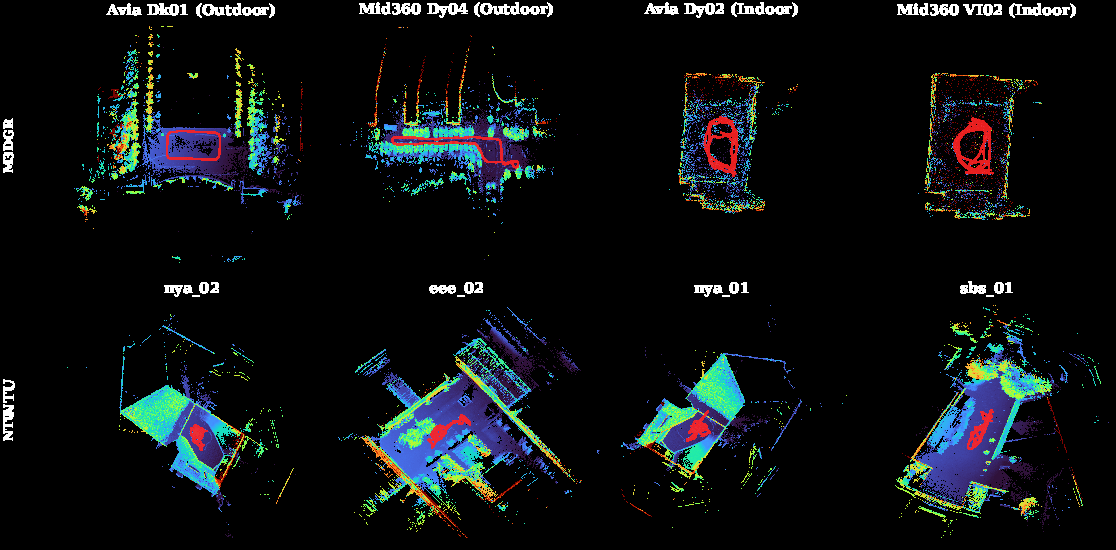
\includegraphics[width=\columnwidth]{../figure/20260418/pointcloud_grid_12panel.pdf}
  \caption{Reconstructed point cloud maps with estimated trajectories
  (red). Row~1: M3DGR Avia Dk01 / Mid-360 Dy04 (outdoor), Avia Dy02 /
  Mid-360 VI02 (indoor). Row~2: NTU VIRAL (nya\_02, eee\_02, nya\_01,
  sbs\_01). Height-colored BEV.}
  \label{fig:map}
\end{figure}

\textbf{FOV-aligned divergence patterns}
(Fig.~\ref{fig:fov_paired}). Each indoor bag contains simultaneous
Avia and Mid-360 data; while this paired design controls for
trajectory and environment, it does not fully isolate FOV from
confounded factors such as point density, surface observability, and
sensor-class noise. The observed pattern is nonetheless consistent
with FOV-driven degeneracy as the dominant cause: the 70\textdegree{}
FOV yields 4--5$\times$ fewer correspondences and 40--50\% of frames
exhibit $\ge 3$ degenerate directions, while Mid-360 exhibits zero
degenerate frames throughout, and these rank-deficiency events
co-occur with baseline divergence onset: across the 8 indoor Avia bags
and three baselines with logged trajectories (FAST-LIO2, iG-LIO,
Point-LIO), median time to first \SI{1}{\meter}/\SI{5}{\meter}/\SI{10}{\meter}
position error is \SI{1.3}{\second}/\SI{5.4}{\second}/\SI{10.9}{\second}
(p95 \SI{1.9}{\second}/\SI{8.0}{\second}/\SI{30.5}{\second}). All baselines invert the information matrix
without eigenvalue-based projection; under narrow FOV, rank deficiency
amplifies null-space noise and corrupts the map within
\SIrange{10}{15}{\second}, whereas HD-LIO's eigenvalue decomposition,
cached surfel normals, and $\sigma^2_n$ weighting jointly prevent this
cascade. Per-group Wilcoxon vs the strongest baseline (Bonferroni-corrected,
$\alpha_\mathrm{corr}{=}0.0125$): NTU vs LIO-SAM
$p_\mathrm{raw}{=}3.9{\times}10^{-3}$, 95\% CI $[+7,{+}22]$\,mm
(\textbf{significant}); Avia outdoor vs Faster-LIO $3.9{\times}10^{-2}$,
CI $[-13,{+}60]$\,mm (n.s.); Mid-360 indoor vs FAST-LIO2 $7.8{\times}10^{-2}$,
CI $[+1,{+}3]$\,mm (n.s.). Indoor Avia is outside the framework
(baseline ATEs unmeasurable on diverged runs).

\begin{figure}[t]
  \centering
  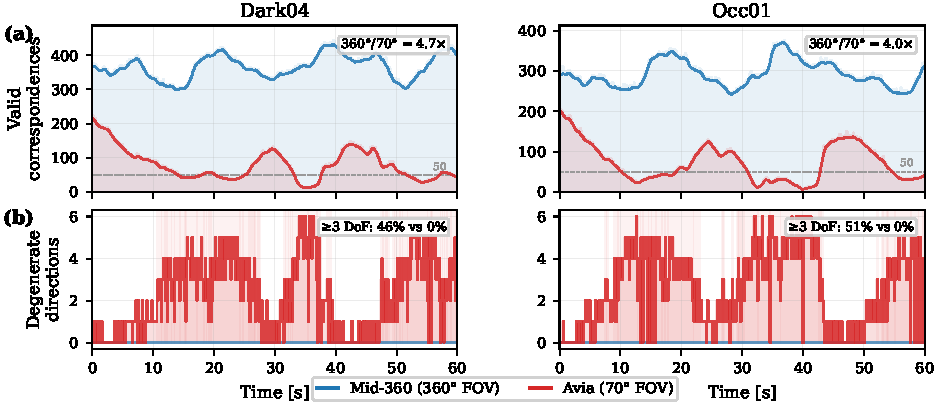
\includegraphics[width=\columnwidth]{../figure/indoor_avia/fov_paired_comparison.pdf}
  \caption{Paired FOV-aligned comparison on Indoor Dark04 and Occ01.
  Both sensors share the same robot trajectory and environment, with
  FOV being the dominant differing factor (residual differences in
  point density, observability, and sensor noise are not fully
  controlled).
  (a)~Valid correspondence count: the 70\textdegree{} FOV yields
  4--5$\times$ fewer correspondences than 360\textdegree{}.
  (b)~Degenerate direction count: 40--50\% of Avia frames exhibit
  $\geq$3 rank-deficient DoFs, while Mid-360 exhibits none.}
  \label{fig:fov_paired}
\end{figure}

\subsection{Timing}
HD-LIO runs at \SI{8.3}{\milli\second} mean per scan on a single core
(AMD Ryzen~5 5600), well within the \SI{100}{\milli\second} budget at
\SI{10}{\hertz} scan rate. For context, FAST-LIO2 reports
$\approx$\SI{5}{\milli\second}~\cite{xu2022fastlio2},
Faster-LIO \SIrange{3}{5}{\milli\second}~\cite{bai2022fasterlio},
DLIO \SIrange{3}{7}{\milli\second}~\cite{chen2023dlio}, and
iG-LIO \SIrange{8}{12}{\milli\second}~\cite{chen2024iglio}
(all on comparable Intel i7 / AMD~Ryzen hardware).
HD-LIO's overhead relative to FAST-LIO2 stems from the dual-source
correspondence lookup and incremental surfel map update; the
$6{\times}6$ eigendecomposition for degeneracy detection adds
$<$\SI{0.1}{\milli\second}. Peak memory is $\approx$450\,MB
(vs.\ $\approx$200\,MB for FAST-LIO2), attributed to the three-level
hash maps and the co-resident PVMap ring buffer.

\subsection{Ablation Study}\label{sec:ablation}

TABLE~\ref{tab:ablation_avia} provides per-mechanism ablation on M3DGR
Avia (70\textdegree{} FOV) and Mid-360 (360\textdegree{} FOV),
isolating each contribution across complementary geometric regimes.

\begin{table}[t]
  \centering
  \caption{Ablation: ATE RMSE [\si{\meter}] on M3DGR Avia (70\textdegree{}) and
  Mid-360 (360\textdegree{}). Underline = full system. The three
  per-sequence columns are deliberately chosen \emph{regime extremes}
  (dynamic / corridor degeneracy) and their arithmetic mean does not
  equal $\overline{\mathrm{ATE}}_9$, which is the average over all
  nine sequences. Each ablation row disables one mechanism from the
  sensor-specific configuration used in
  TABLE~\ref{tab:m3dgr_outdoor}.}
  \label{tab:ablation_avia}
  \small
  \resizebox{\columnwidth}{!}{%
  \begin{tabular}{@{}lccccccccccc@{}}
    \toprule
    & \multicolumn{5}{c}{Avia (70\textdegree{} FOV)} & & \multicolumn{5}{c}{Mid-360 (360\textdegree{} FOV)} \\
    \cmidrule{2-6} \cmidrule{8-12}
    Config & Dk01 & Dy03 & VI03 & $\overline{\mathrm{ATE}}_9$ & $\Delta$ & & Dk01 & Dy03 & VI03 & $\overline{\mathrm{ATE}}_9$ & $\Delta$ \\
    \midrule
    Full            & \underline{0.114} & \underline{0.170} & \underline{0.608} & \underline{\textbf{0.293}} & ---
                    & & \underline{0.150} & \underline{0.169} & \underline{1.003} & \underline{\textbf{0.297}} & --- \\
    w/o degen.\ fb. & 0.162 & 1.293 & 0.724 & 0.449 & +53\%
                    & & 0.151 & 0.169 & 0.969 & 0.297 & +0\% \\
    w/o $\sigma^2_n$ & 0.146 & 0.166 & 1.304 & 0.394 & +34\%
                    & & 0.157 & 0.163 & 1.117 & 0.301 & +1\% \\
    w/o surfel      & 0.121 & 0.158 & 1.018 & 0.377 & +29\%
                    & & 0.152 & 0.164 & 1.240 & 0.845 & +185\% \\
    w/o L2          & 0.135 & 0.652 & 1.079 & 0.432 & +48\%
                    & & 0.156 & 0.164 & 1.087 & 0.295 & $-$1\% \\
    \bottomrule
  \end{tabular}}%
\end{table}

The ablation reveals a clear FOV-dependent regime separation. On
\textbf{Avia} (TABLE~\ref{tab:ablation_avia}, left), degeneracy
feedback is the most impactful (+53\% with removal, $0.293{\to}0.449$\,m,
Dy03 $\times 7.6$), followed by L2 (+48\%, Dy03 $\times 3.8$),
$\sigma^2_n$ (+34\%, VI03 $\times 2.1$), and surfel (+29\%, VI03
$\times 1.7$): the ranking reflects the dominance of
information-geometric corrections under narrow FOV. On
\textbf{Mid-360} (TABLE~\ref{tab:ablation_avia}, right), in contrast,
degeneracy feedback, $\sigma^2_n$, and L2 each show $\le$2\% mean
impact, while surfel removal causes +185\% ($0.297{\to}0.845$\,m),
driven by OC03 diverging to \SI{4.923}{\meter} ($\times 26.6$);
excluding this outlier, surfel impact drops to +8\%. The surfel map
thus plays a dual role: modest accuracy gain on routine sequences,
but critical divergence prevention under severe occlusion regardless
of FOV.

%----------------------------------------------------------------------
\section{Discussion and Conclusion}\label{sec:discussion}
%----------------------------------------------------------------------

\textbf{FOV dependence.} HD-LIO's improvement scales inversely with FOV
completeness: 22\% on OS1-16 (vs.\ LIO-SAM), 26\% on Avia (vs.\
FAST-LIO2), and 5\% on Mid-360 (vs.\ iG-LIO). When 360\textdegree{}
FOV eliminates degeneracy, feedback contributes minimally; when
vertical resolution is sparse (OS1-16), $\sigma^2_n$ dominates; when
FOV is narrow (Avia), both are critical. The indoor paired comparison
corroborates this regime separation: Mid-360 HD-LIO matches baselines
(\SI{0.150}{\meter}), while on Avia in the \emph{same} environments
all baselines diverge and HD-LIO maintains \SI{0.524}{\meter} — a
qualitative gap, divergence versus bounded drift, in a regime where
narrow-FOV sampling yields effective rank $\le 3$ in 40\% of frames.

\textbf{Failure modes.}
On VI03 (908\,m corridor, 17\,min), sustained planar geometry makes
(S1) quantitatively marginal: median $I_d{=}0.18$ along the
longitudinal direction (vs.\ $1.4$ on outdoor sequences), and 18\% of
frames violate (S2). Theorem~\ref{thm:uub} therefore does not apply
unconditionally over this trajectory; on the $82\%$ of frames where
(S2) holds, the bound from~\eqref{eq:vinf} predicts a UUB radius of
${\approx}0.5$\,m, while the remaining $18\%$ of frames contribute an
unmodeled drift increment that accumulates over the 10{,}268-frame
trajectory and produces the observed
\SI{0.608}{\meter} ATE. Surfel, $\sigma^2_n$, and L2 removal each
degrade by $\times$1.7--2.2 here, while degeneracy feedback shows
only $\times$1.2, indicating that under the weakest (S1) regime the
contraction mechanism reaches its assumption-limited regime: the
mechanism is operating where designed, but the assumption violation
fraction sets a hard lower bound on achievable accuracy.

\textbf{Conclusion.}
HD-LIO formalizes the drift-map positive feedback loop as a
per-direction linearized recursion, derives conditions for ultimate
boundedness, and instantiates a three-mechanism intervention on a
hierarchical surfel map with eigenvalue-perturbation-derived
per-correspondence weights. It achieves \SI{0.203}{\meter} mean ATE on
35 baseline-comparable sequences, 22\% below LIO-SAM on NTU~VIRAL, and
is the only method to maintain bounded error on the 8~indoor Avia
sequences (70\textdegree{}) where all six baselines diverge.
Future work: iterative motion undistortion and temporal surfel
invalidation.

\footnotesize
\bibliographystyle{IEEEtran}
\bibliography{refs}

\end{document}
